%! program = pdflatex
\documentclass[12pt]{article}
\usepackage{geometry}
\geometry{a4paper} % or letter or a5paper or ... etc
% \geometry{landscape} % rotated page geometry
\usepackage{amsmath,amssymb,setspace,fancyhdr,geometry,url}
\usepackage{graphicx,caption}
\usepackage{lscape,amsthm}
\usepackage{gensymb}
\usepackage{bm}
\usepackage[authoryear,round]{natbib}
%\usepackage{subcaption}
\RequirePackage{lineno}
\usepackage{titlesec}

\allowdisplaybreaks[1]
\allowbreak

\renewcommand{\thesection}{}
\renewcommand{\thesubsection}{}
\titleformat{\section}{\Large\bfseries}{\thesection}{0em}{}
\titleformat{\subsection}{\large}{\thesubsection}{1em}{}

\title{Quantifying Spatio-Temporal Variation of Invasion Spread}
\author{Joshua Goldstein$^1$, Murali Haran$^{1*}$, Ottar N. Bj$\o$rnstad$^2$ and Andrew Liebhold$^3$}
\date{}
\begin{document}
\linenumbers
\doublespacing
\label{firstpage}

\maketitle

\noindent$^1$Department of Statistics, Pennsylvania State University, University Park, PA 16802 USA\\
{*}email: mharan@stat.psu.edu\\
$^2$Departments of Entomology and Biology, Pennsylvania State University, University Park, PA 16802 USA\\
$^3$US Forest Service Northern Research Station, Morgantown, WV 26505 USA

\begin{center} {\bf Word count: 4630} \end{center}

\clearpage

\begin{abstract}\noindent
\begin{itemize}
\item The spread of invasive species can have far reaching environmental and ecological consequences. Understanding invasion spread patterns and the underlying process driving invasions are key to predicting and managing invasions.
\item We develop a set of statistical methods to characterize local spread properties and demonstrate their application using historical data on the spread of the gypsy moth, {\it Lymantria dispar}, and hemlock wolly adelgid, {\it Adelges tsugae}. Our method uses a Gaussian process fit to the surface of waiting times to invasion in order to characterize the vector field of spread.
\item Using this method we estimate with statistical uncertainties the speed and direction of spread at each location. Simulations from a stratified diffusion model verify the accuracy of our method.
\item We show how we may link local rates of spread to environmental covariates for our two case studies.
\end{itemize}
\end{abstract}

\begin{center}{\bf Key-words:} Gaussian processes, Bayesian statistics, biological invasions,\\ gypsy moth, hemlock wolly adelgid, \texttt{R} package \end{center}

\clearpage

\section{Introduction}\label{sec:intro}

When a non-native species successfully establishes in an exotic environment it enters the spread phase of biological invasions during which it expands its range into suitable habitat \citep{lockwood2013invasion}. Ecological theory has shown that the speed of invasion spread is a joint function of the dispersal rate and the population growth rate of the invading species \citep{skellam1951random,okubo1980diffusion}; any habitat characteristic that influences population growth or dispersal can thus influence the rate of spread. Rates of spread may vary considerably among species and for a given species, spread rates may vary across heterogeneous landscapes \citep{shigesada1987speeds, tobin2007invasion}. Understanding the mechanisms causing heterogeneity in the rate of invasion spread is key to predicting future rates of spread and to identifying important locations for management.

In this work we develop new methods for estimating local speed and dominant direction of spread along the invasion front. Our approach can be applied to identify statistically significant environmental and geographic determinants of local invasion rates.

In addition to environmentally-driven heterogeneity in rates of spread, there is considerable variation among species in the extent to which invasion spread is continuous. Spread of some species occurs via continuous expansion of the range into contiguous areas. For example, the North American muskrat, {\it Ondatra zibethica}, invaded central Europe from 1905-1927 via gradual expansion of its range in concentric circles \citep{skellam1951random}.  The spread of other species is highly discontinuous, characterized by a pattern referred to as �stratified diffusion� \citep{shigesada1995}; following initial establishment, expansion may happen with long-range jumps into isolated uninvaded areas, founding new colonies which expand and eventually coalesce to form a contiguously invaded zone. This pattern is observed in many species of invading organisms, such as invasion of North America by the Argentine ant, {\it Linepithema humile} \citep{suarez2001patterns} and the gypsy moth, {\it Lymantria dispar} \citep{sharov2002slow}.

Quantifying the spread of non-native species and relating invasion speed to habitat heterogeneity is important for predicting and managing biological invasions. Several methods have been developed for measuring spread based upon fitting range size to time since establishment or estimating spread by directly quantifying displacement of range boundaries over time \citep{sharov1997methods,tobin2007comparison,gilbert2010comparing}.  These methods are generally well-suited for quantifying average spread range and temporal variation therein, but they are limited in their ability to quantify local spread rates and their relation to local habitat characteristics.  Also, these methods are generally designed to quantify spread as a continuous process; identification of long-range jumps in stratified dispersal is usually done visually in a non-automated fashion. These gaps in existing methodology provides our motivation for developing new and statistically rigorous methods for estimating local speed and direction of spread. We take advantage of recent statistical theory on the estimation of spatial gradients. We test our methods on simulated data generated from a stratified diffusion model and apply them to two detailed case studies of biological invasions, the historical spread of the gypsy moth and the hemlock wolly adelgid, {\it Adelges tsugae}, in North America.


\section{Data} \label{sec:data}

\subsection{Gypsy moth}

Native to Europe and Asia, the gypsy moth was accidentally introduced from France to Massachusetts in the late 1860's \citep{liebhold1989learning}, it has since spread throughout much of the northeastern US. The gypsy moth is now established in a large area composed of the north Atlantic states and bordering Canadian provinces, as well as a second focus resulting from a long-range jump event to Michigan around 1980 \citep{liebhold1992gypsy,johnson2006allee,tobin2007invasion}.

The invasion of the gypsy moth across North America has been rather slow compared to the rate of spread of many other alien species \citep{liebhold2008population}. Mean spread was estimated at 21 km per year from 1960 to 1990 \citep{liebhold1992gypsy}. The relatively slow rate of spread can be attributed, in part, to the fact that females of North America populations are flightless. Gypsy moth populations spread by short-range windborne dispersal of $1^{\text{st}}$ instar larvae through a process known as `ballooning' \citep{mason1981larval}. Egg masses are also accidentally transported on wood or human-made objects, forming new colonies ahead of the invasion front and resulting in a pattern of stratified diffusion \citep{sharov2002slow}.

The full invasion history of the gypsy moth in the US is reflected in the year of government designation of gypsy moth quarantine by county. County-level quarantine records for gypsy moth are maintained by the United States Department of Agriculture (U.S. Code of Federal Regulations, Title 7, Chapter III, Section 301.45). Historically, an entire county was usually designated part of the quarantined area when established gypsy moth populations were first detected anywhere within the county. These records are updated annually and exist from 1934 to the present. From 1900 to 1934, the year when counties were first infested has been described in various other published sources \citep[e.g.,][]{ burgess1913report, burgess1915report, liebhold1992gypsy}.  As additional covariates, we used county-level data \citep{liebhold1997gypsy} on the percent of the forest basal area comprised of oaks, which is a favored food plant of the gypsy moth, and the size (km$^2$) of each county.



\subsection{Hemlock wolly adelgid}

Hemlock woolly adelgid (HWA) is an insect species responsible for mass defoliation of its host trees, eastern hemlock and Carolina hemlock \citep{orwig2002landscape,morin2009anisotropic}. Native to East Asia, it was first discovered in the USA in Virginia in the 1950s \citep{ward2004eastern}.  HWA life stages can be transported by wind, wildlife, especially birds, and humans. Since its discovery, it has gradually expanded its range into much of the northeastern USA \citep{evans2007geographically,morin2009anisotropic}. By 1969 it was found in southern Pennsylvania and it invaded southern New England by 1985, spreading at an estimated speed of 20-30 km/year \citep{morin2009anisotropic}.

As with the gypsy moth, historical spread of the HWA was recorded at the county level. Records from the US Forest Service Forest Health Protection are available for 1951, 1971, 1981, 1996, and from 2001 to 2011.   We use the basal area of hemlock \citep{morin2004mapping} and plant hardiness zone \citep{cathey1990usda} for each county as additional covariates for our analysis.


\section{Methods} \label{sec:methods}

Previous estimates of spread for gypsy moth data have estimated rates averaged over space. \cite{liebhold1992gypsy} estimated spread rates for five geographic regions by the slope of a least-squares regression of time on distance to a reference point in each region. Spread rates have also been estimated by measuring the average displacement of range boundaries over time \citep{sharov1997methods,tobin2007comparison}.

Previous research on estimating spatial gradients from georeferenced biological data has focused on detecting zones or boundaries of rapid change across space using geostatistical {\it wombling} \citep{womble1951}. Wombling methods involve estimating local vector gradients by fitting bilinear functions over a lattice of points. This method has been applied to genetic \citep{barbujani1989detecting} as well as ecological \citep{fortin1994edge} data. More recent wombling methods for areal data feature Bayesian hierarchical spatial models in order to identify significant boundaries after accounting for spatial dependence via Markov random fields \citep{banerjee2004hierarchical,fitzpatrick2010,lu2007bayesian}, with applications to ecology and epidemiology.

The use of spatial gradients to estimate biological spread is motivated by the fact that if the surface is the waiting time to first appearance, then the reciprocal of the gradient length is a measure of the invasion speed: Fast spread leads to shallow waiting time surfaces, while slow spread results in steep surfaces. Previously \cite{johnson2004landscape} estimated spread gradients using thin plate spline applied to waiting times (as measured by wavelet phase angles) to study outbreak dynamics of the larch budmoth. \cite{farnsworth2009} used a similar spline surface approach to study spread of avian influenza. The thin plate spline approach yielded gradients which reflect the magnitude and direction of the spread, a simple general-purpose approach for visualization, but has not associated errors with local spread estimates which prevents rigorous inference regarding whether, for example, any observed spatial variation is statistically significant.

\subsection{Gaussian process gradient models} \label{sec:models}

\cite{banerjee2003directional} developed theory for estimating gradients of an arbitrary surface by specifying a Gaussian process model directly for the spatial gradients. We take advantage of this because when the gradients are defined on the waiting times to first appearance, the reciprocal of the gradient will represent the rate of spread.

We develop methods to rigorously test important features of the invasion, following existing theory \citep{banerjee2003directional,banerjee2006bayesian}. Below we further describe pattern recognition methods for detecting sites of long-range dispersals, radial expansion and directional patterns in historical spread. We also provide, in an electronic supplement, computer code for an R \citep{ihaka1996r, rmanual2013} software package that automates inference about spread.

We assume we have observations of the year of first appearance $\bm{Y} = \{ Y(\bm s_1),...,Y(\bm s_n) \}$ at locations $\{ \bm s_1,...,\bm s_n \}, \bm s_i \in \mathbb{R}^2$. For our examples, data are county-level quarantine records and the spatial locations $\{ \bm s_1,..,\bm s_n \}$ are taken to be the centroids of counties for the gypsy moth where $n=571$ counties (Figure \ref{fig:first}a) and for the HWA where $n=340$ counties (Figure \ref{fig:first}b). Coordinates are projected using the Albers equal area conic projection with standard parallels $29^{\degree}30'$ and $45^{\degree}30'$. For county $i$, $Y(\bm s_i)$ is the year the county was added to the quarantine. We assume $Y(\bm s)$ can be modelled using an isotropic Gaussian process with mean $\mu(\bm s)$ and covariance $K(\cdot)$.

\cite{banerjee2003directional} defines the finite difference directional derivative process at location $\bm s$ for scale {\it h} in direction $\bm u$ as
\[
Y_{\bm{u},h}(\bm{s}) = \dfrac{ Y(\bm{s} + h\bm{u}) - Y(\bm{s}) }{ h }
\]
where $\bm u$ is a unit vector. The directional derivative process in direction $\bm u$ is then defined as
\[
D_{\bm{u}} Y(\bm{s}) = \displaystyle\lim_{h \rightarrow 0} Y_{\bm{u},h}(\bm{s})
\]
assuming the mean square limit exists. Of interest is the gradient of $Y(\bm s)$ at $\bm{s}$, the vector of directional derivatives
\[
\nabla Y(\bm{s}) = \left( D_{\bm{e_1}} Y(\bm{s}), D_{\bm{e_2}} Y(\bm{s}) \right)
\]
in orthonormal basis directions $\bm{e_1} = (1,0)$ and $\bm{e_1} = (0,1)$. \cite{banerjee2003directional} shows there exists a joint trivariate Gaussian process for $Y(\bm{s})$ and $\nabla Y(\bm{s})$, and therefore $\bm Y$ and $\nabla \bm Y = \{ \nabla Y(\bm s_1),...,\nabla Y(\bm s_n) \}$ have a joint multivariate normal distribution which takes the form
\[
\left( \begin{array}{c}
\textbf{Y} \\
\nabla \textbf{Y} \\
\end{array} \right) \sim
N_{3n} \left[
\left( \begin{array}{c}
\boldsymbol{\mu} \\
\nabla \boldsymbol{\mu} \\
\end{array} \right),
\left( \begin{array}{cc}
K(D) & -\nabla K(D) \\
\nabla K(D)^T & -H_K(D) \\
\end{array} \right)
\right]
\]
where $D$ is the $n \times n$ matrix of pairwise Euclidean distances of \textbf{s}, and $K(D)$ represents the $n \times n$ matrix of $K(\cdot)$ applied element-wise to $D$. $\nabla \boldsymbol{\mu}$ is the length $2n$ vector
\[
\bigg( \dfrac{ \partial{\mu} }{ \partial{x} }(s_1),...\dfrac{ \partial{\mu} }{ \partial{x} }(s_n),\dfrac{ \partial{\mu} }{ \partial{y} }(s_1),...,\dfrac{ \partial{\mu} }{ \partial{y} }(s_n) \bigg)^T,
\]
$\nabla K(D)$ is the $n$ x $2n$ matrix
\[
\left( \begin{array}{cc}
\dfrac{\partial{K}}{\partial{x}}(D) &  \dfrac{\partial{K}}{\partial{y}}(D) \\
\end{array} \right),
\]
and $H_K(D)$ is the $2n$ x $2n$ matrix
\[
\left( \begin{array}{cc}
\dfrac{\partial^2{K}}{\partial{x^2}}(D) &  \dfrac{\partial^2{K}}{\partial{x}\partial{y}}(D) \\
\dfrac{\partial^2{K}}{\partial{x}\partial{y}}(D) & \dfrac{\partial^2{K}}{\partial{y^2}}(D) \\
\end{array} \right).
\]
The conditional distribution of the gradient is therefore given by
\[
\nabla \textbf{Y} | \textbf{Y},\Theta \sim
N_{2n} \left(
\nabla \boldsymbol{\mu} - \nabla K(D)^T [K(D)]^{-1} (\textbf{Y} - \boldsymbol{\mu}), -H_K(D) - \nabla K(D)^T [K(D)]^{-1} \nabla K(D) \right).
\]
where $\Theta$ is a vector of mean and covariance parameters for the Gaussian process. Letting $\delta = (s_0-s_1,...,s_0-s_n)$, the estimated gradient at a point $s_0$ is given by
\begin{equation}
\begin{split}
\nabla Y(s_0) | \textbf{Y},\Theta \sim
N_2 \big(
\nabla \mu(s_0) - \nabla K(\delta)^T [K(D)]^{-1} (\textbf{Y} - \boldsymbol{\mu}), \\
-H_K(0) - \nabla K(\delta)^T [K(D)]^{-1} \nabla K(\delta) \big).
\label{eq:gradpred}
\end{split}
\end{equation}
Note that for the gradient process to be well-defined, the original process must be mean square differentiable and all second order partial derivatives of $K$ must exist. This is the case, for instance, when $K$ is chosen to belong to the Matern family with smoothness parameter $\nu > 1$ \citep{stein1999interpolation}.

For our applications, we assume the original process $Y(\bm s) = \mu(\bm s) + w(\bm s) + \epsilon(\bm s)$, with mean function  $\mu(\bm s) = \beta_0 + \beta_1 s_x + \beta_2 s_y$, correlated spatial error $w(\bm s) \sim GP(0, K(\cdot))$ with Mat\'ern covariance smoothness $\nu = 3/2$, which takes the explicit form $K(r)=\sigma^2 (1+\phi r) \text{exp}\{-\phi r\}$, and uncorrelated error $\epsilon(\bm s) \sim N(0,\tau^2)$, where $\tau^2$ is a nugget effect capturing both mesurement error and microscale variability.

We infer the mean and covariance parameters $\Theta = ( \beta_0, \beta_1, \beta_2, \sigma^2, \phi, \tau^2 )$ based on a Bayesian approach using a Markov chain Monte Carlo (MCMC) algorithm. Flat prior distributions are assumed for mean parameters and inverse gamma priors are assumed for the partial sill $(\sigma^2)$ and nugget $(\tau^2)$ with shape parameter $2$ and scale parameter set to an approximate value from the empirical semivariogram. For the range $(\phi)$ a uniform prior is chosen with a support that allows the process to vary from low to high dependency. Simulation from the predictive distribution of the gradient can then be done by composition; given each posterior sample of $\Theta$, a sample for $\nabla Y(s_0)$ can be drawn from (\ref{eq:gradpred}).

At a given location $s_0$, posterior samples are the gradient at $s_0$ in the $x$ and $y$ directions. When the data are times of first appearance, steeper gradients correspond to slower speeds. Therefore posterior estimates of the gradient (including Bayesian credible intervals) allow us to make inferences on the local speed and dominant direction of spread. Therefore the speed of spread is the inverse of the magnitude of the posterior gradient $\| \nabla Y(s_0) \|$, and the dominant direction of the spread is in the direction of the gradient $\nabla Y(s_0) / \| \nabla Y(s_0) \|$.


\subsection{Detecting sources and long-range jumps}\label{sec:longrange}

It is useful to have automated methods to identify candidate locations for foci of long-range jumps ahead of the advancing front as different from locations with contiguous ``wave-like'' diffusive spread. However, consistently identifying these foci is a challenge. We have identified two candidate solutions. The first borrows methods from circular statistics, and the second is a more direct test of the average gradient orthogonal to a curve around the point.


The Rayleigh test \citep[see e.g.][]{jammalamadaka2001topics} is a statistical test of whether a circular distribution is random or non-random. When applied to the vectors of spread near a point, a non-random distribution implies a unified directional spread through that point. We take directions of spread in a neighborhood around each centroid and test if these directions are drawn from a uniform circular distribution. Say we have $n$ estimated directional vectors of spread $x_i, y_i$ in a neighborhood around a point. Let $r$ be the length of the mean vector from this sample, $r = \sqrt{\bar{x}^2 + \bar{y}^2}$. The test statistic is given by $R = 2 nr^2$ for the test of \\
\indent $H_0:$ Directional vectors are distributed randomly \\
\indent $H_a:$ Directional vectors are distributed non-randomly. \\
Under the null hypothesis $R$ will be $\chi^2$ distributed with $2$ degrees of freedom. If the test fails to reject the null this may contribute evidence that the directional distribution is uniform as would be the case for radial spread from the point. While this may occur because the location is the point source of a long-range jump, the Rayleigh test will also flag areas with vectors that are converging {\it to} the point (akin to an ecological sink) or are truly random. Therefore while it is useful for flagging potential sites of long-range jumps, it is not a perfect method because we need to visually distinguish between the three different scenarios that all lead to failure to reject the null.

We also test directly the distribution of the gradient around a point, which will allow us to check if there is significant radial expansion around that point.

Define a curve $\mathcal{C}_{t^*} = \{ s(t): t \in [0,t^*] \}$, where $s(t) = \left( s_1(t), s_2(t) \right) \in \mathcal{R}^2$ and $s'(t)$ is the componentwise derivative. Let $\eta(s(t))$ be the unit vector normal to the curve at the point $s(t)$. The total gradient normal to $\mathcal{C}_{t^*}$ is
\[
\Gamma(t^*) = \int_0^{t^*} \langle \nabla Y(s(t)), \eta(s(t)) \rangle dv,
\]
where $v$ is the arc-length of the curve, $v(t^*) = \int_0^{t^*} \| s'(t) \| dt$, and so
\[
\Gamma(t^*) = \int_0^{t^*} \langle \nabla Y(s(t)), \eta(s(t)) \rangle \| s'(t) \| dt,
\]
In \cite{banerjee2006bayesian} it is shown that the distribution for the total gradient over a curve is a Gaussian process on $[0,T]$, $\Gamma(t^*) \sim GP( \mu_\Gamma(t^*), K_\Gamma(\cdot, \cdot) )$ with
\[
\mu_\Gamma(t^*) = \int_0^{t^*} \langle \mu(s(t)), \eta(s(t)) \rangle \| s'(t) \| dt
\]
\[
K_\Gamma(t_1^*, t_2^*) = \int_0^{t_1^*} \int_0^{t_2^*} \eta^T(s(t_1)) H_K\left[ s(t_2) - s(t_1) \right] \eta(s(t_2)) \| s'(t_1) \| \| s'(t_2) \| dt_1 dt_2
\]
where $\mu(\cdot)$ is the mean of the original process $Y(s)$ and $H_K(\cdot,\cdot)$ is the hessian of the covariance of $Y(s)$. \\

The conditional distribution of interest is
\[
\Gamma(t^*) | \textbf{Y},\Theta \sim N\big( \mu_\Gamma - \gamma^T_\Gamma(t^*) [K(D)]^{-1} (\textbf{Y} - \boldsymbol{\mu}),
K_\Gamma(t^*, t^*) - \gamma^T_\Gamma(t^*) [K(D)]^{-1} \gamma_\Gamma(t^*) \big)
\]
where for $j = 1,...,n$
\[
\gamma^T_\Gamma(t^*)_j = \text{cov}( \Gamma(t^*), Y(s_j) ) = \int_0^{t^*} \langle K \left[ s(t) - s(j) \right], \eta(s(t)) \rangle \| s'(t) \| dt.
\]
The terms $\gamma_\Gamma(t^*)$ and $K_\Gamma(t^*, t^*)$ are not available analytically, and must be computed using numerical integration. The {\it average} gradient normal to the curve $\mathcal{C}_{t^*}$ is simply the total gradient $\Gamma(t^*)$ divided by the arc-length.

Using this method centered on each location we can test the gradient normal to four sides of a box with sides of length $r$. As an heuristic we say if the spread is significantly {\it out} of at least two sides of the box, and does not go significantly {\it into} any side of the box, we will flag the location as a potential site of a long-range jump. We do this for a grid over the region of interest. In our figures, red lines indicate sides where there is a significant outward spread.


\subsection{Driving factors of spread}

We can gain insight into the mechanisms of spread by relating the geographic variation in spread to characteristics of habitat. To account for spatial dependence we fit a Bayesian spatial regression model to log-speeds of spread speed using the $\texttt{R}$ package {\it spBayes} \citep{spBayes}. We apply the log transformation to the response since the speeds have right-skewed distributions. If the mean speed at location $\bm s_0$ is given by $V(\bm s_0)$, then we assume
\[
\text{log} V(\bm s_0) = X^T(\bm s_0) \bm\beta + w(\bm s_0) + \epsilon(\bm s_0)
\]
where $X( \bm s )$ is a vector of the spatially varying environmental and geographical covariates of interest. $w(\bm s) \sim GP(0,G(\cdot))$, $G(\cdot)$ has Mat\'ern covariance smoothness with smoothness $\nu$, range $\phi$ and partial sill $\sigma^2$ and $\epsilon(\bm s) \sim N(0,\tau^2)$. Priors are selected as before and joint estimation is done via MCMC for  $\{ \bm\beta, \sigma^2, \phi, \tau^2, \nu \}$.

\section{Results}\label{sec:results}

\subsection{Gypsy moth}

Significant speeds and directions of historical spread of the gypsy moth are plotted at the locations of each county in the quarantine in Figure \ref{fig:mothspread}a. The mean speed of spread over all counties is 20.8 km/year, with a median of 13.4 km/year.  Distributions for the magnitude of spread at each location tend to be right skewed, where the average length of 95\% credible intervals is 29.7 km/year.

In Figure \ref{fig:mothspread}b we test for sites of long-range dispersals using the two methods discussed above. For each method in practice we take circular neighborhoods of $1^{\circ}$. Points identified by the Rayleigh test are marked in black in Figure \ref{fig:mothspread}b, along with boxes where the gradient test is significant. Both methods identify three potential sites around the northeastern coast, Michigan and central-western Pennsylvania. Prior analysis confirms two of these sites, as the population was first introduced in Massachusetts in the 1860s and a discrete population was later established in Michigan \citep{liebhold1992gypsy}. A close look at Figure \ref{fig:first}a also highlights the jump to Centre County, PA in the mid 1970s.

We relate speed of spread to latitude and longitude, quarantine date, county size, and finally the percent basal area of trees preferred as hosts of the gypsy moth. Estimated parameters of the spatial regression model are given in Table \ref{table:regression}a. We verify that on average the gypsy moth spread faster as it moved west. We also found that basal area of susceptible host trees is significantly associated with speed of spread, consistent with the concept that local growth rates will be larger in the face of more favorable habitat, and should consequently enhance invasion spread rates.



\subsection{Hemlock woolly adelgid}

Significant speeds and directions of spread for the HWA are plotted at each county in Figure \ref{fig:hwaspread}a. We find a mean speed of spread of 20.5 km/year across counties, with a median speed of 13.5 km/year. The $95\%$ credible intervals for spread at each location have an average length of 31.8 km/year.

Sites of long-range dispersal events are identified in Figure \ref{fig:hwaspread}b. We detect areas of apparent long-range dispersals in Richmond and southern PA, suggesting a pattern of stratified diffusion. \cite{morin2009anisotropic} also found that expansion is significantly influenced by availability of host trees. Low winter temperatures can cause extensive mortality in HWA populations and limit expansion to the north \citep{trotter2009variation}. Therefore we relate speeds of spread to environmental features including the presence or absence of hemlock trees, and the average plant hardiness zone for each county, an index based on the mean annual minimum winter temperature \citep{cathey1990usda}. Estimates from the regression model are given in Table \ref{table:regression}b. We observed evidence that historically expansion is faster to the west and north. We also find as in \cite{morin2009anisotropic} that spread is significantly associated with the abundance of host trees. We also tested the interaction between plant hardiness zone and latitude and found at a given latitude, HWA spread significantly slower through areas with lower plant hardiness zones $[ \beta = 3.4 (0.4, 6.3) ]$.


\subsection{Simulation}

We tested the ability of our method to recover the effects that spatially varying habitats have on the speed of spread. To accomplish this, data are simulated from a stratified diffusion model following \cite{shigesada1995}. Stratified diffusion is a combination of neighborhood diffusion and long distance dispersal. As the size of the original colony expands, new colonies are more likely to be created by long distance migrants.

The simulation starts with a single colony, centered at the initial point of invasion. The occupied area grows out in a circle, the radius $r$ growing at constant rate $c$. This colony can then form offspring colonies from long-distance migrants in a random direction at a distance $L$ from the invasion front. New colonies form at a rate $\lambda(r)$ that is a function of the colony radius. These offspring colonies grow at speed $c$ and form offspring colonies of their own.

We begin with an initial introduction in Massachusetts in the year 1900. Colony range expansion $c$ varies by longitude to simulate a slow period of initial expansion; $c=10$ km/year east of $-78^{\degree}$ and $c=20$ km/year west of $-78^{\degree}$. New colonies form at rate $\lambda(r) = 0.1 r$ a distance $L=10$ km from the invasion front. Additionally, to mimic the observed Gypsy Moth data an artificial long-range jump is introduced in Michigan in 1950. The simulation is run for 107 years with an annual timestep.

The time until the invasion front reaches each county is recorded as the simulated quarantine data (Figure \ref{fig:simspread}a). In Figure \ref{fig:simspread}b we observe that our method of inference has successfully identified the two fixed colony introductions as regions of long-range jumps. We recover mean spread rates in the west of 10.7 km/year and in the east of 21.4 km/year, close to the actual values used in the simulation.


\section{Discussion}\label{sec:discussion}

To study the establishment and spread of biological invasions we present a new method to estimate local rates and direction of spread, and identify key spatial features including sources, sites of rapid spread and long-range jumps. We visualize and make inferences on historical patterns of spread of the gypsy moth and hemlock woolly adelgid as well as validate the methodology on simulated data. Posterior inference in a Bayesian setting allows us to test the significance of spread patterns and spatial features of these invasions in a rigorous way.

Taking our local estimates of gypsy moth spread and averaging them across time yields results in line with previous estimates in the literature \citep{liebhold1992gypsy}. We find an average speed of 11.4 km/year across counties quarantined from 1900 to 1915, followed by a slow spread (5.0 km/year) across counties from 1916 to 1965 and then a period of very rapid expansion (25.8 km/year) from 1966 to 2000. These changes may also be related to the differences in Allee effects among different regions along the invasion front as evidenced in \cite{tobin2009role}. From 2000 to present, coincident with the ``Slow the Spread'' program of control \citep{sharov2002slow} we observed an average speed of 14.6 km/year.

Our estimates for the spread of HWA when spatially averaged are also in line with estimates from the literature (e.g. \cite{ward2004eastern}). There is evidence that HWA range expansion is limited both by a lack of host trees and in the north by extreme winter temperatures. We also observe the spread of HWA to appear less diffusive than the gypsy moth. One explanation for this is the important role of wildlife, especially migratory birds, as a mechanism for HWA dispersal \citep{mcclure1990role} in addition to windborne dispersal and human transport, which also accounts for anisotropy in spread observed in \cite{morin2009anisotropic}.

Our abilities to identify patterns of spread are constrained by the spatial and temporal resolution of our data. County-level quarantine data are typically coarser than, for example, gypsy moth pheromone trap count data, though \cite{tobin2007comparison} showed the two sources of gypsy moth data provided similar estimates. Additionally, the original Gaussian process must be sufficiently smooth for a gradient process to exist (we take the Matern model with smoothness parameter $\nu=3/2$), with the consequence that some information is lost at small scales. We rely for the most part on annual records, but before 2001 the range of HWA was recorded at less frequent intervals. This is a potential source of bias in our early estimates of HWA spread.

For large spatial datasets, fitting a Gaussian process is a computational burden. Once the original Gaussian process is fit, however, we can draw samples by composition from the gradient process quickly. When the number of spatial locations is in the thousands we must likely have to rely on approximations such as the predictive process model of \cite{banerjee2008gaussian}.

Generally whenever the data are point-referenced waiting times, the speeds of spread can be estimated from the inferred gradient process. Therefore the methods presented here are generally applicable in ecology and epidemiology to spread of invasive species and infectious disease. These methods are also potentially applicable to non-invasion problems such as population waves such as the spread of an advantageous allele \citep{fisher1937wave}, or recurrent outbreak waves in species such as the larch bud moth \citep{johnson2004landscape}. An \texttt{R} package that automates the inference is available as an electronic supplement.


\section{Acknowledgements}

This work has been funded by the Bill and Melinda Gates Foundation and by the National Science Foundation, \#DEB-1354819.

\section{Data Accessibility}

We will put the data in the DRYAD data repository (www.datadryad.org).

\clearpage

\bibliographystyle{apalike}
\bibliography{references}

\clearpage

\begin{table}
\centering
\caption{Results of a spatial regression of speeds of spread (km/year) for the gypsy moth (a) and hemlock wolly adelgid (b) including posterior means and 95\% credible intervals obtained using the highest posterior density interval algorithm \citep{chen2000hpd}.}
\begin{tabular}{c|c}
{\bf (a) Gypsy Moth} & $\beta$ \\
\hline
Intercept & $-1.6 (-11.0,9.3)$ \\
Longitude & $-5.1 (-8.1,-2.2)$ \\
Latitude & $-2.3 (-6.6,1.2)$ \\
County size & $-0.00007 (-0.00020,0.00002)$ \\
Quarantine date & $0.0006 (-0.0044, 0.0056)$ \\
Basal\% susceptible trees & $0.0023 (0.0000, 0.0042)$ \\
\hline
{\bf (b) HWA} & $\beta$ \\
\hline
Intercept & $19.5 (3.1,36.6)$ \\
Longitude & $-9.8 (-14.9,-4.8)$ \\
Latitude & $8.5 (1.7,16.0)$ \\
Quarantine date & $-0.003 (-0.009,0.003)$ \\
I$_{\text{presence of hemlock}}$ & $0.09(0.01,0.07)$ \\
Plant hardiness zone & $0.014 (-0.19,0.23)$ \\
\end{tabular}
\label{table:regression}
\end{table}

\clearpage

\begin{figure}
\centering
\caption{Year of first appearance by county for the gypsy moth (a) and hemlock woolly adelgid (b).}
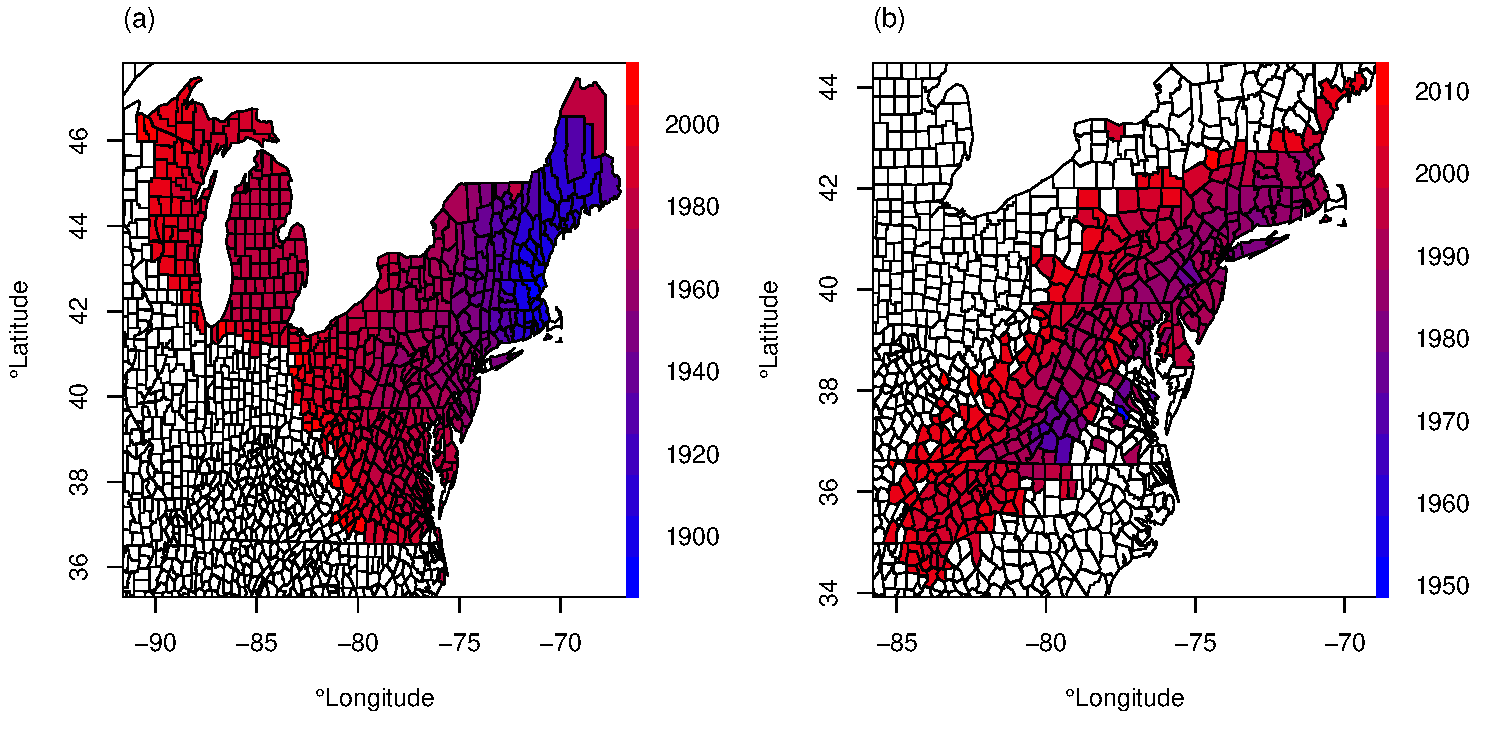
\includegraphics[width=\textwidth]{figures/firstappearance}
\label{fig:first}
\end{figure}


\begin{figure}
\centering
\caption{(a) Patterns of spread of the gypsy moth. Arrows indicate local speeds and directions of spread, and are plotted where spread is significant. (b) Identifying long-range jumps for the gypsy moth invasion. Black points are potential sites of long-range jumps identified by the Rayleigh test. Red boxes around a point indicate regions of potential long-range jumps identified by the grid search method (lines indicate sides of a box around a potential source where the spread was significantly out of the box).}
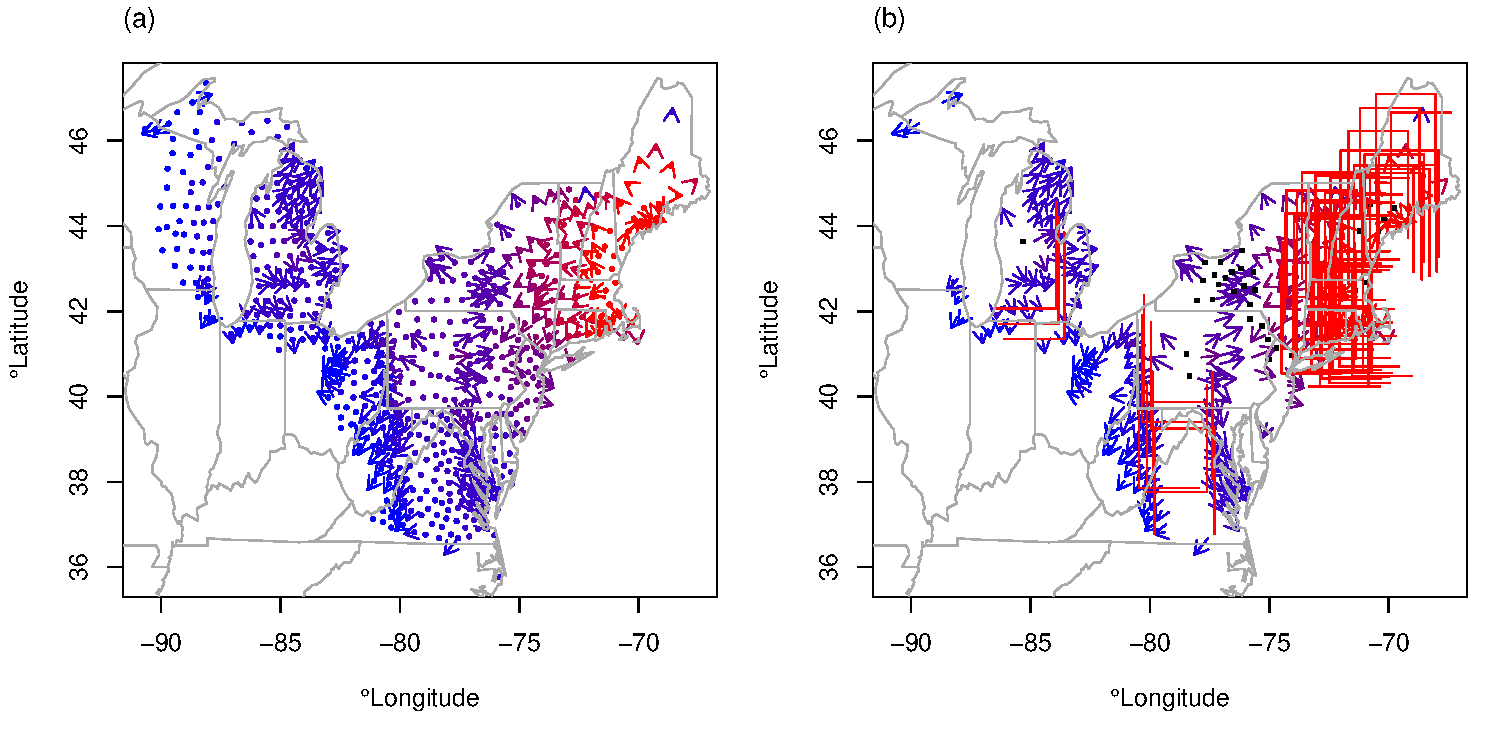
\includegraphics[width=\textwidth]{figures/MothSpread}
\label{fig:mothspread}
\end{figure}


\begin{figure}
\centering
\caption{(a) Patterns of spread of the hemlock wolly adelgid. Arrows indicate local speeds and directions of spread, and are plotted where spread is significant. (b) Identifying long-range jumps for the gypsy moth invasion. Black points are potential sites of long-range jumps identified by the Rayleigh test. Red boxes around a point indicate regions of potential long-range jumps identified by the grid search method (lines indicate sides of a box around a potential source where the spread was significantly out of the box).}
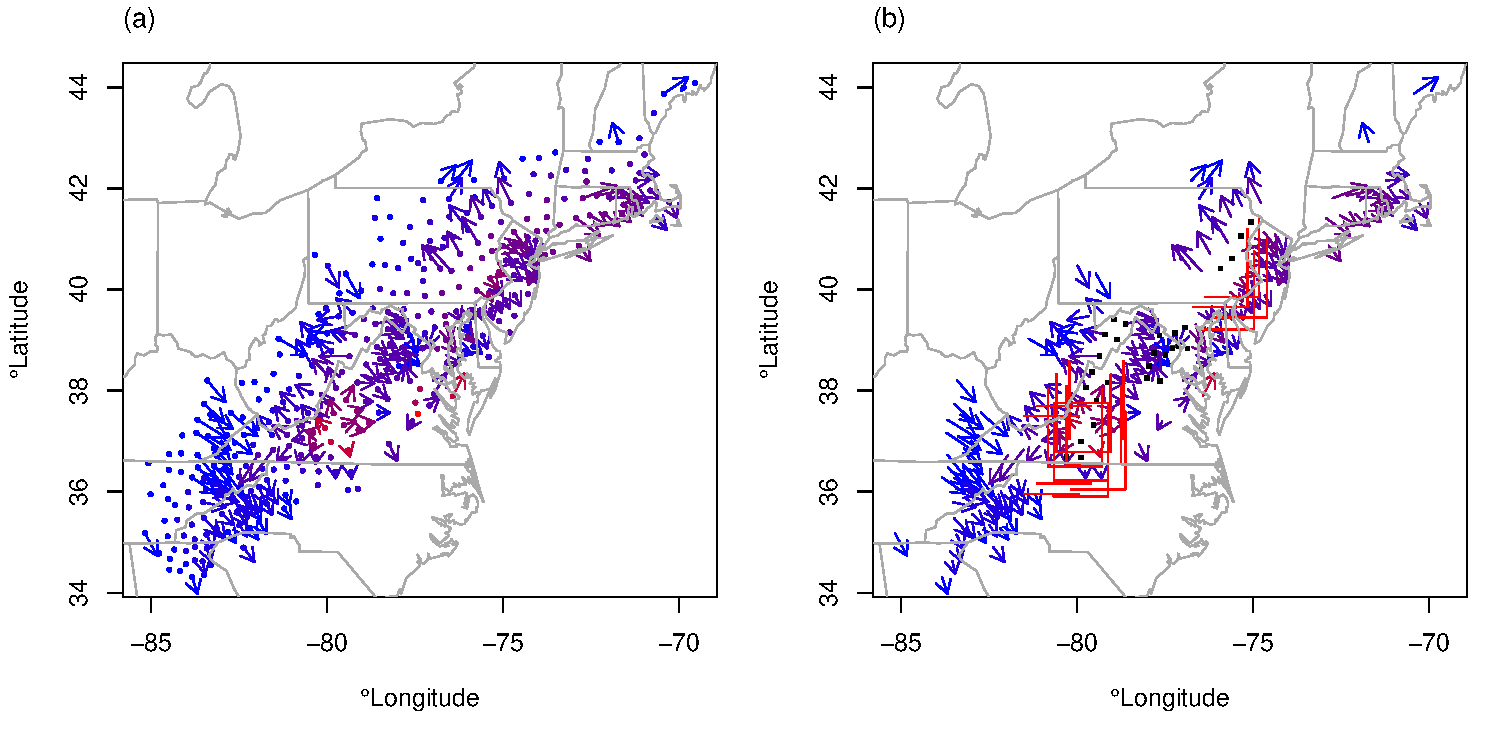
\includegraphics[width=\textwidth]{figures/HWASpread}
\label{fig:hwaspread}
\end{figure}


\begin{figure}[h!]
\centering
\caption{(a) Waiting times of the stratified diffusion simulation following \cite{shigesada1995}. (b) Long-range jumps for the simulated invasion. Black points are potential sites of long-range jumps identified by the Rayleigh test. Red boxes around a point indicate regions of potential long-range jumps identified by the grid search method.}
\label{fig:simspread}
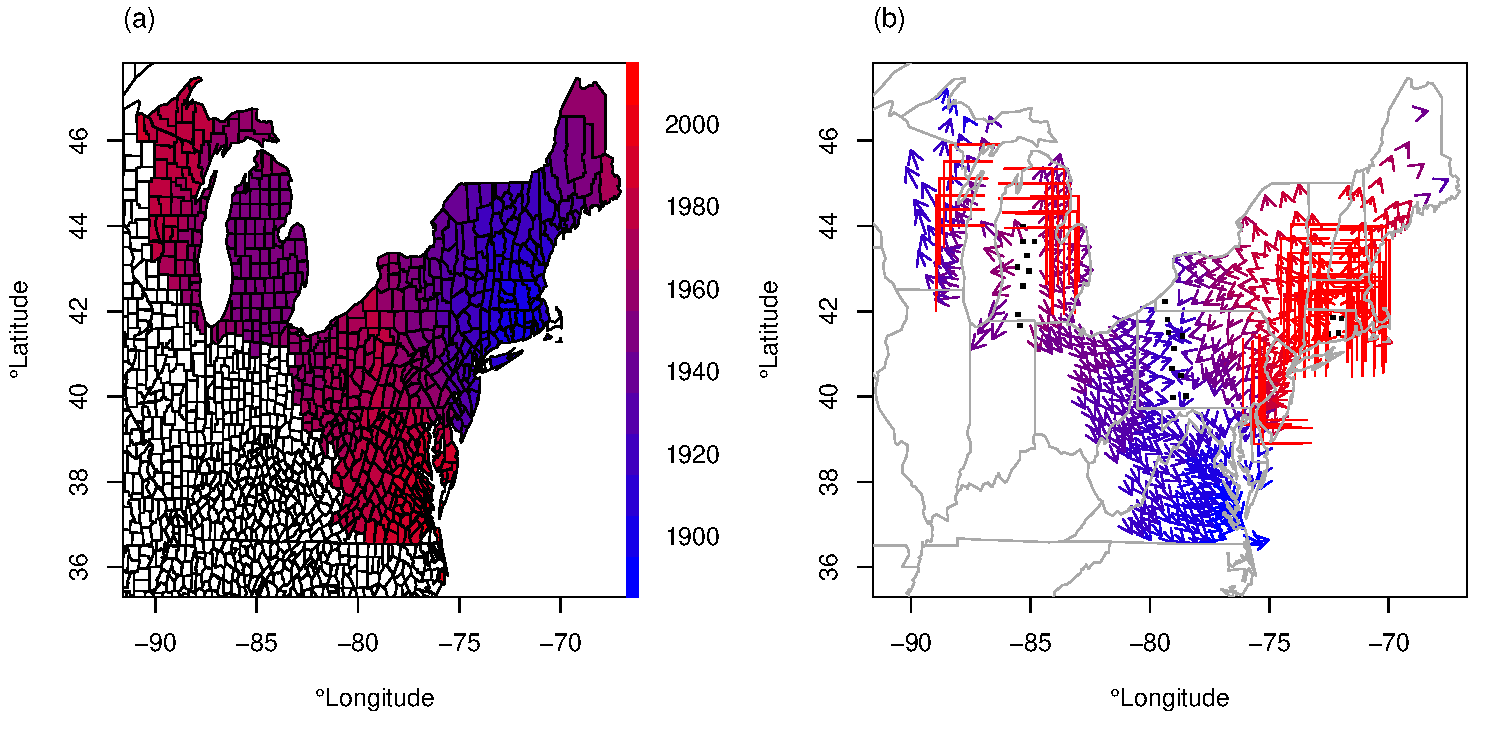
\includegraphics[width=\textwidth]{figures/SimSpread}
\end{figure}

\label{lastpage}
\end{document}